\documentclass[11pt,a4paper]{article}

% --- Packages ---
\usepackage[utf8]{inputenc}
\usepackage[T1]{fontenc}
\usepackage{graphicx}
\usepackage{booktabs}
\usepackage{hyperref}
\usepackage[margin=2.5cm]{geometry}
\usepackage{caption}
\usepackage{subcaption}
\usepackage{xcolor}
\usepackage{float}

\title{UbiLife: Data Exploration and Preparation\\[0.3em]
\large Mobile Sensing at UbiComp/ISWC 2025}
\author{}
\date{}

\begin{document}
% ============================================================
% Title Page
% ============================================================
\begin{titlepage}
\centering

% --- University name at top ---
\vspace*{1cm}

\includegraphics[width=0.4\textwidth]{images/dtu.png}~\\[1cm]
{\large\scshape Technical University of Denmark\par}
\vspace{0.3cm}
{\normalsize Department of Health Technology\par}

\vspace{0.5cm}
\rule{\textwidth}{0.4pt}

% --- Title ---
\vspace{2cm}
{\Huge\bfseries Sense-making of\\[0.3em] Raw Mobile Sensing Data\par}
\vspace{1cm}
{\Large Mobile Sensing at UbiComp/ISWC 2025\par}

\vfill

% --- Author ---
{\Large Miklos Havlik\par}
\vspace{0.3cm}
{\large Student number: s240069\par}

\vspace{1.5cm}

% --- Supervisors ---
\begin{tabular}{rl}
\textbf{Supervisors:} & Jakob Eyvind Bardram (\href{mailto:jakba@dtu.dk}{jakba@dtu.dk}) \\
                       & Nigel Sj\"olin Grech (\href{mailto:nsjgr@dtu.dk}{nsjgr@dtu.dk}) \\
\end{tabular}

\vspace{1.5cm}

% --- Date ---
{\large March 4, 2026\par}
\vspace{1cm}

\end{titlepage}

% ============================================================
\section{Background}
% ============================================================
UbiComp/ISWC is a well-known international conference where researchers, designers, developers, and practitioners gather to share and discuss new work in ubiquitous, pervasive, and wearable computing~\cite{ubicomp2025}. The 2025 edition took place at Aalto University in Espoo, Finland (October 12–16, 2025), with the main conference running from October 14–16 and pre-conference workshops on October 12–13.

The \textbf{UbiLife} study collected mobile sensing data from around 82 participants, who carried smartphones running the CARP data collection app during the conference period (October 9–29, 2025). The dataset has over one million records across 15 different data streams, which covers passive sensors like step count, activity recognition, and location, as well as device data such as battery state, screen events, and heartbeat (keep alive) signals. It also includes environmental information such as weather and air quality, along with self-reported surveys on stress, sleep, wellbeing, personality, and session ratings. The main goal is to get a better understanding of how people move, behave and feel during a large academic conference, by looking at data collected from multiple sensor sources.

% ============================================================
\section{Data Exploration}
% ============================================================


% ------------------------------------------------------------
\subsection{Sensor Data}
% ------------------------------------------------------------

Table~\ref{tab:streams} summarises the 15~data streams with their record counts and participant coverage.
Figure~\ref{fig:stream_overview} provides a visual overview.

\begin{figure}[H]
\centering
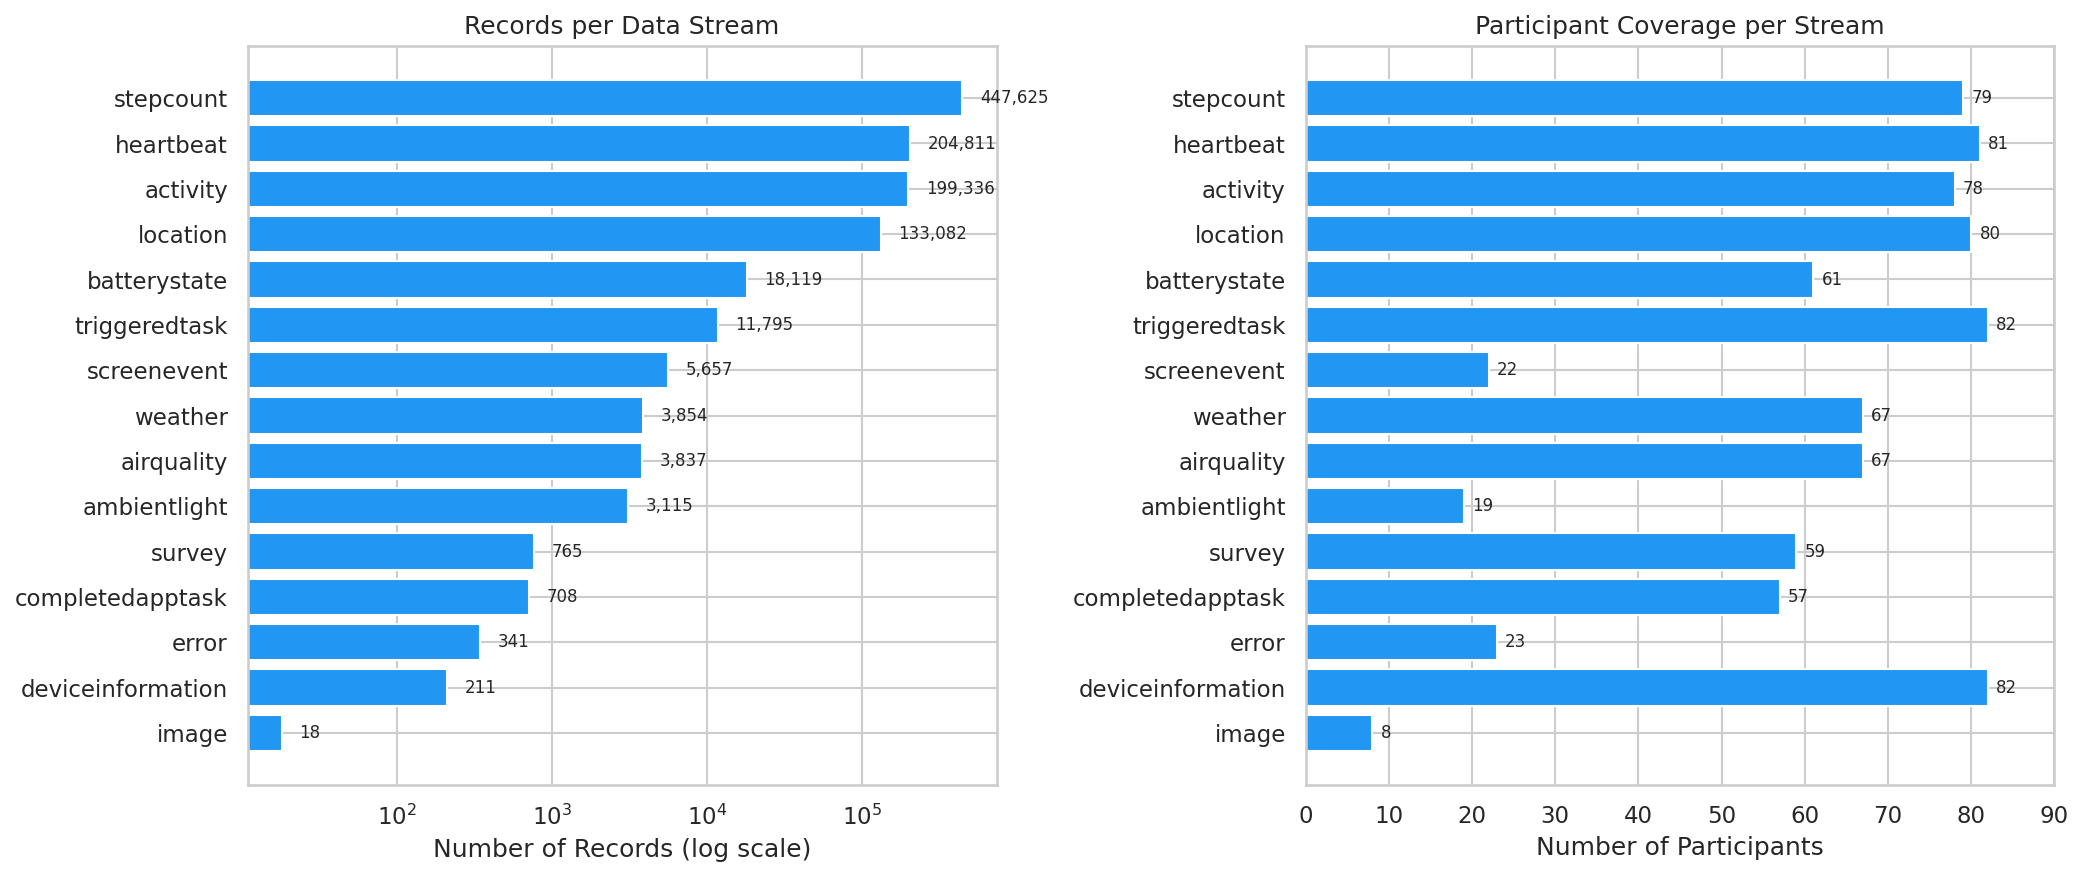
\includegraphics[width=\textwidth]{figures/01_stream_overview.png}
\caption{Overview of record counts and participant coverage across all 15~data streams.}
\label{fig:stream_overview}
\end{figure}

\begin{table}[H]
\centering
\caption{Record volumes and participant coverage per data stream.}
\label{tab:streams}
\small
\begin{tabular}{lrr}
\toprule
\textbf{Data Stream} & \textbf{Records} & \textbf{Participants} \\
\midrule
Step count      & 447\,625  & 79 \\
Heartbeat       & 204\,811  & 81 \\
Activity        & 199\,336  & 78 \\
Location        & 133\,082  & 80 \\
Battery state   &  18\,119  & 61 \\
Screen events   &   5\,657  & 22 \\
Weather         &   3\,854  & 67 \\
Air quality     &   3\,837  & 67 \\
Ambient light   &   3\,115  & 19 \\
Triggered tasks &  11\,795  & 82 \\
Completed tasks &      708  & 57 \\
Survey          &      765  & 59 \\
Device info     &      211  & 82 \\
Error log       &      341  & 23 \\
Image metadata  &       18  &  8 \\
\bottomrule
\end{tabular}
\end{table}

\subsubsection{Temporal Coverage}

Data collection spans October~9 to 29, with most activity happening during the main conference days (October~13 to 17).
Figure~\ref{fig:heartbeat} shows the heartbeat coverage heatmap: mean coverage during the conference was 33.4\%, and night hours (00:00 to 06:00) had lower coverage across the board.
All times in this report are local conference time (Europe/Helsinki, UTC+3), converted from the UTC timestamps recorded by CARP.
Restricted to the four main conference days (October~13 to 16, Figure~\ref{fig:heartbeat_13_16}), 39~participants reach $\geq$10\% coverage, with a mean of 37.6\%.
There is a large spread in how much data each participant contributed. Some recorded over 30\,000 step count entries while others had fewer than 1\,000 (Figure~\ref{fig:records_per_participant}).

\begin{figure}[H]
\centering
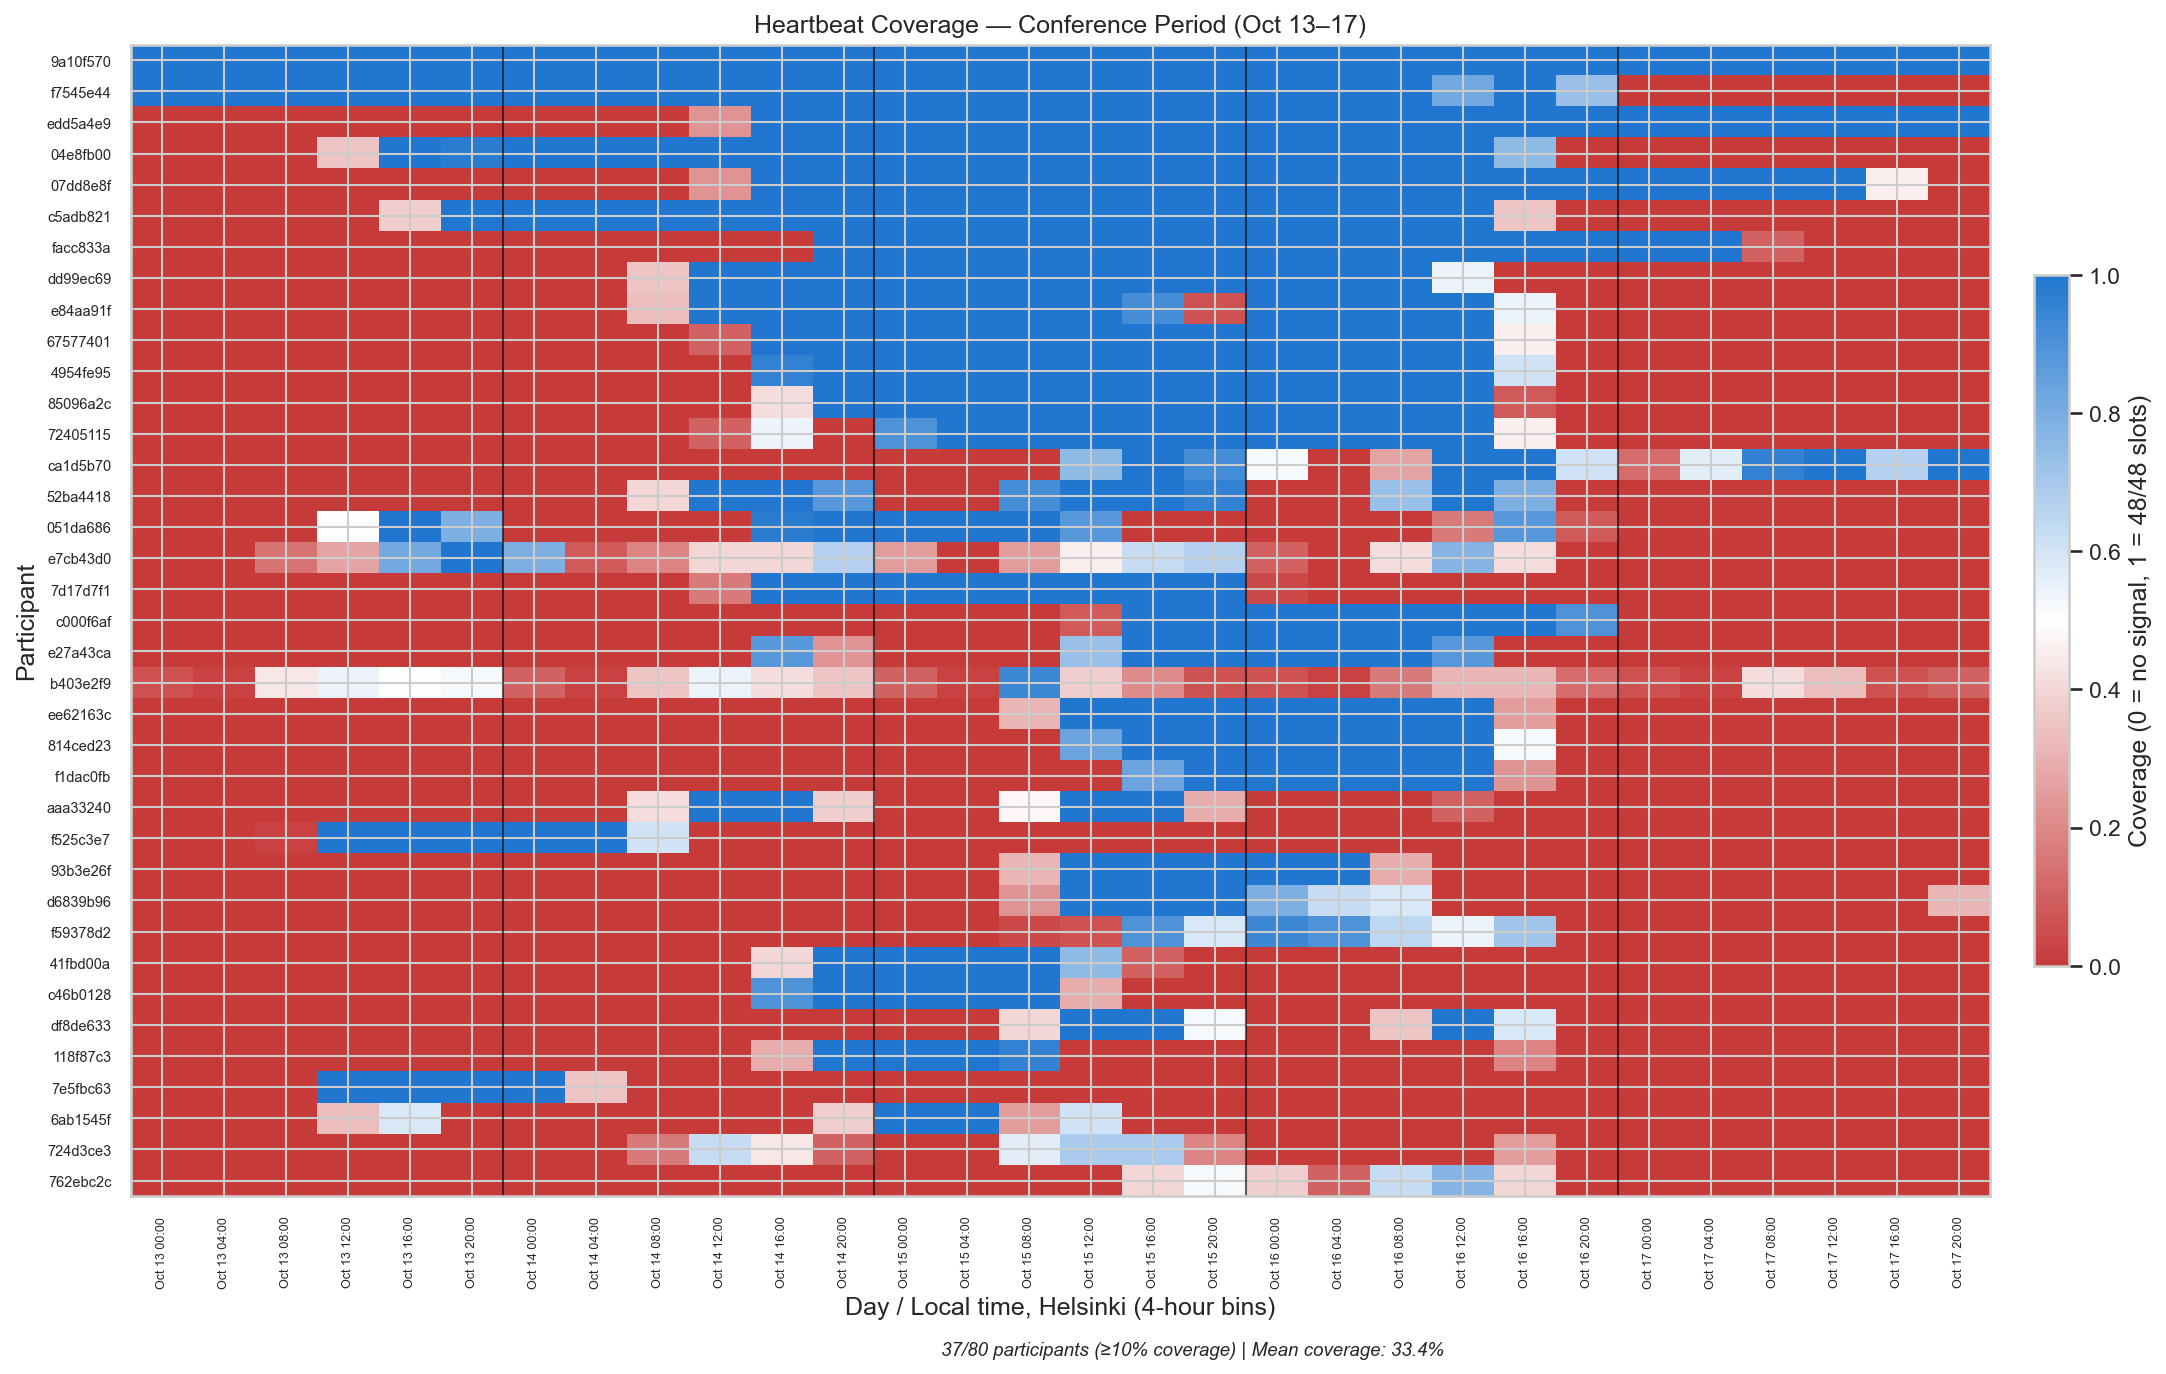
\includegraphics[width=\textwidth]{figures/01_heartbeat_coverage.png}
\caption{Heartbeat coverage heatmap (4-hour bins) for 37~participants with $\geq$10\% coverage during October~13--17. Blue indicates high coverage; red indicates low coverage.}
\label{fig:heartbeat}
\end{figure}

\begin{figure}[H]
\centering
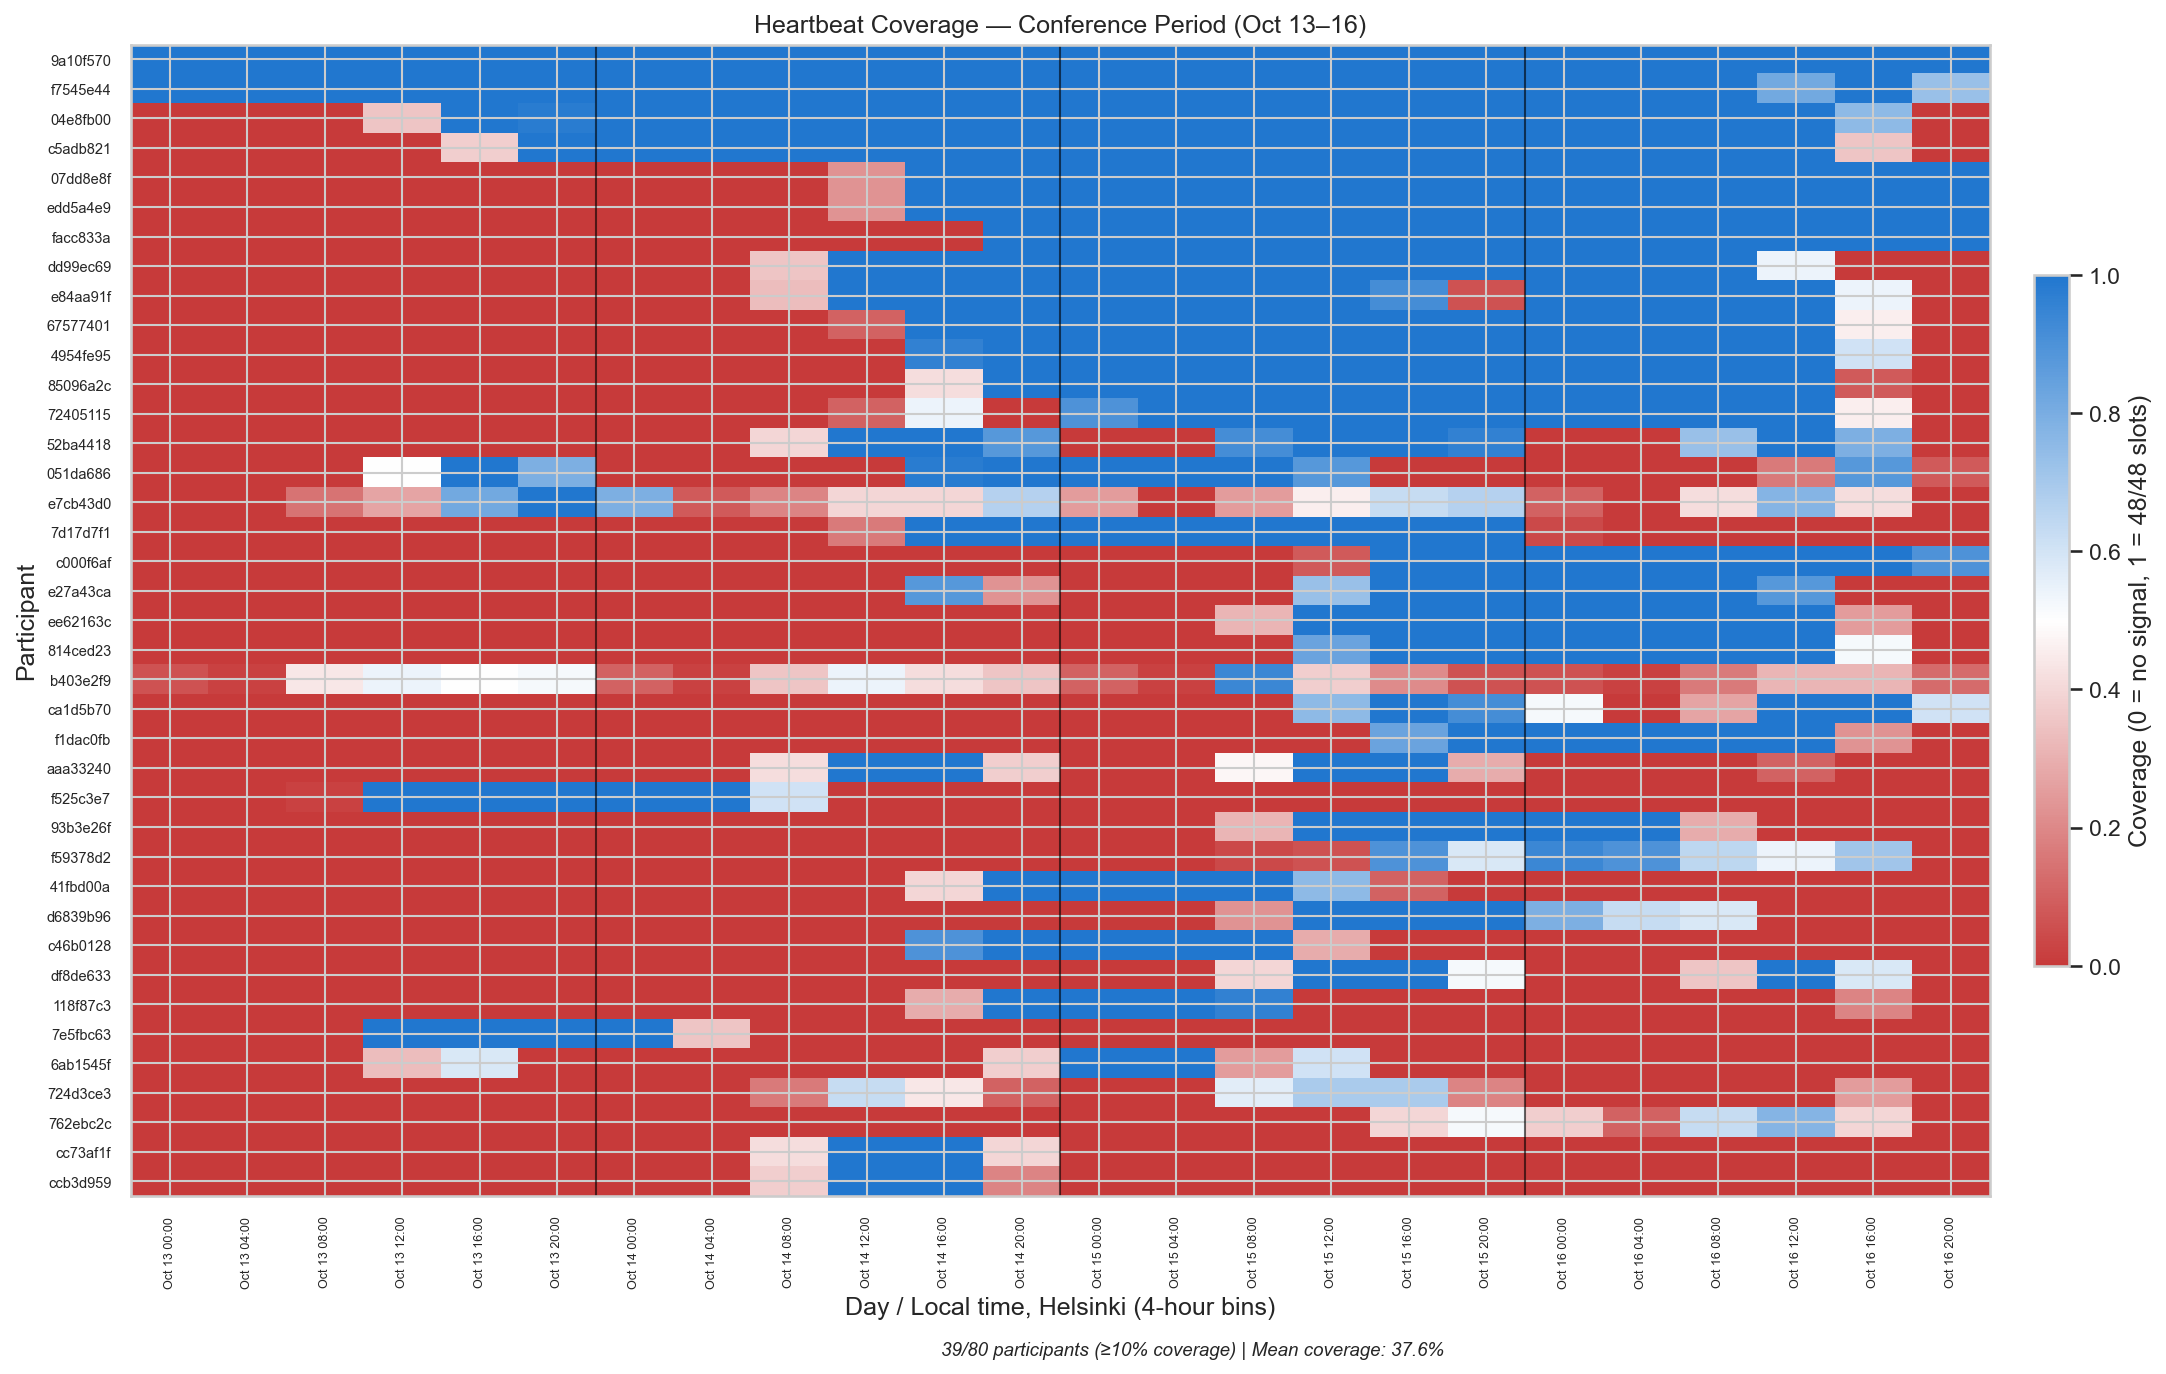
\includegraphics[width=\textwidth]{figures/01_heartbeat_coverage_13_16.png}
\caption{Heartbeat coverage heatmap (4-hour bins, local time) for 39~participants with $\geq$10\% coverage during the main conference days, October~13--16.}
\label{fig:heartbeat_13_16}
\end{figure}

\begin{figure}[H]
\centering
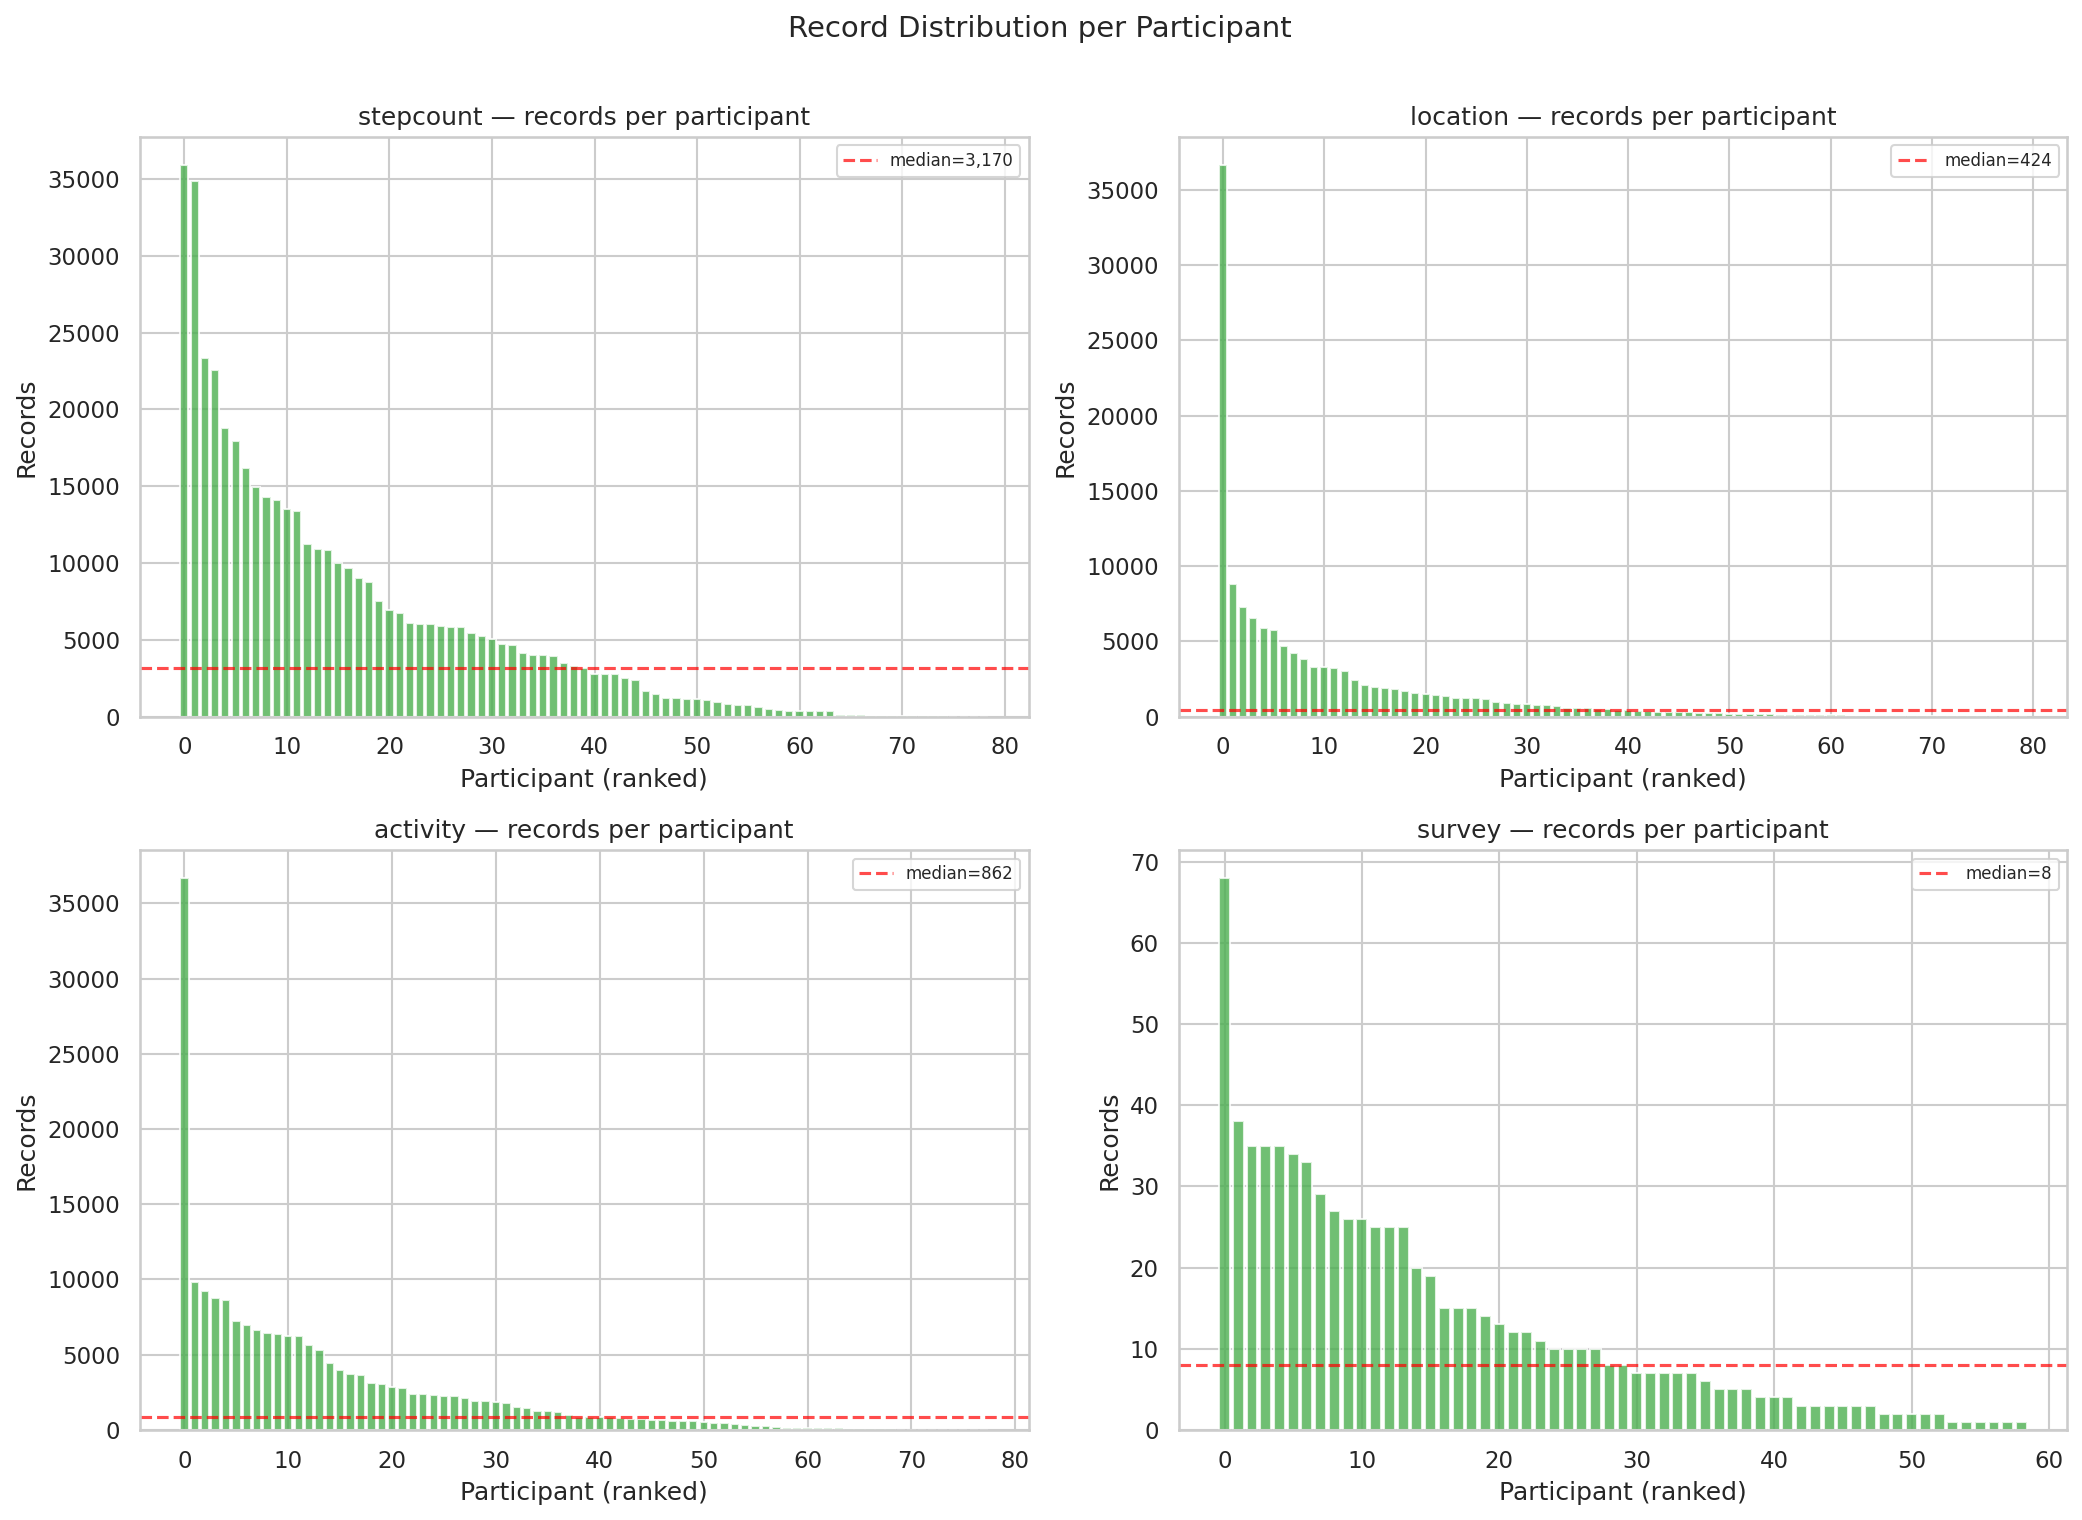
\includegraphics[width=\textwidth]{figures/01_records_per_participant.png}
\caption{Distribution of records per participant across key sensor streams.}
\label{fig:records_per_participant}
\end{figure}

\subsubsection{Activity Recognition}

Five activity types were classified: \textsc{STILL}, \textsc{WALKING}, \textsc{IN\_VEHICLE}, \textsc{RUNNING}, and \textsc{ON\_BICYCLE}.
\textsc{STILL} dominates between 00:00 and 06:00, while \textsc{WALKING} peaks during conference hours (09:00--18:00).
Figure~\ref{fig:activity} shows the overall distribution and hourly patterns.

\begin{figure}[H]
\centering
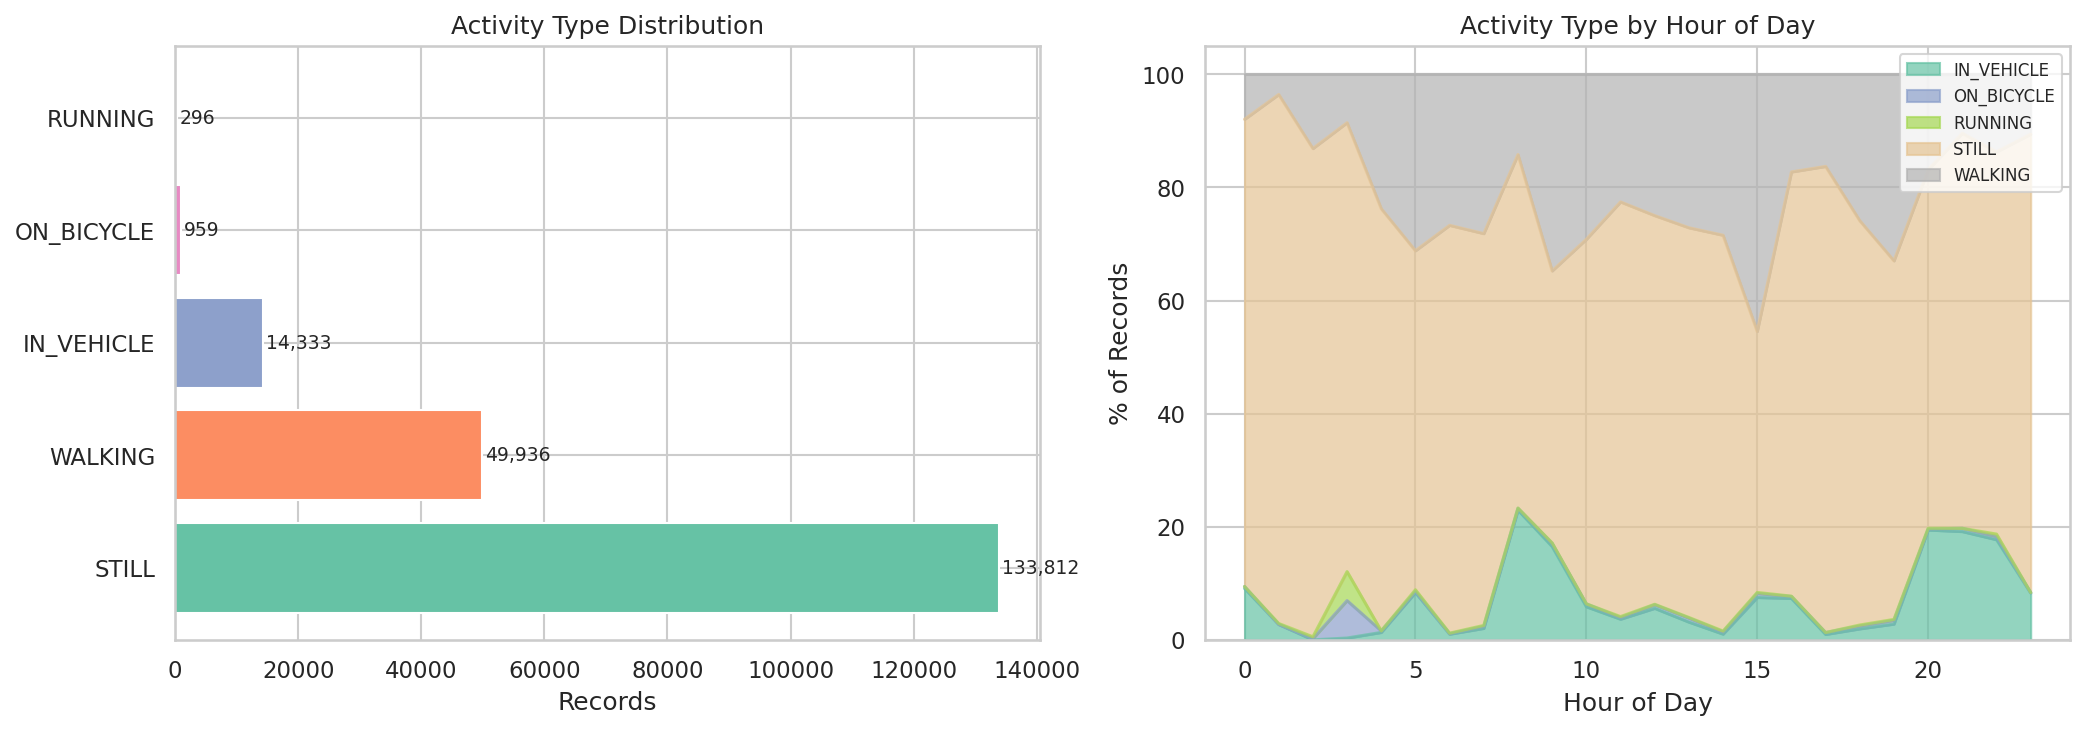
\includegraphics[width=\textwidth]{figures/01_activity_types.png}
\caption{Activity type distribution and hourly activity patterns across all participants.}
\label{fig:activity}
\end{figure}

\subsubsection{Device Diversity}

Both iOS and Android platforms are represented, with manufacturers including Apple, Samsung, and Google (Figure~\ref{fig:devices}).

\begin{figure}[H]
\centering
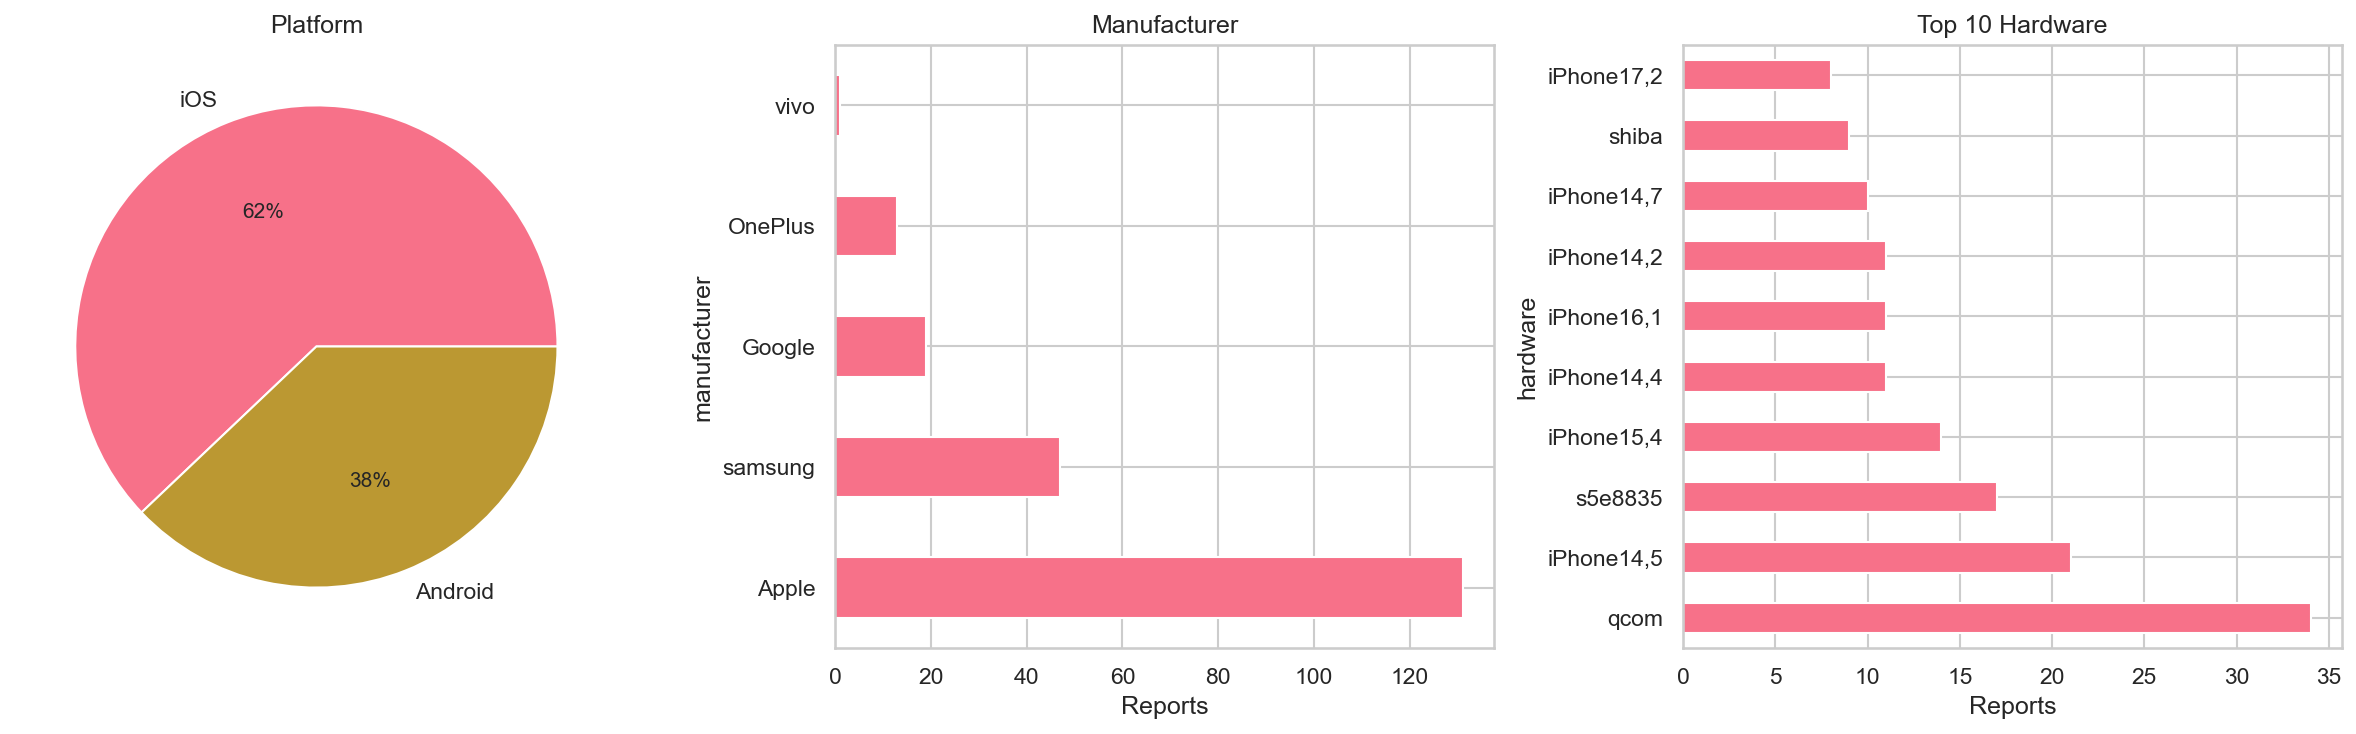
\includegraphics[width=\textwidth]{figures/01_devices.png}
\caption{Device platform, manufacturer, and hardware breakdown.}
\label{fig:devices}
\end{figure}

% ------------------------------------------------------------
\subsection{Survey Data}
% ------------------------------------------------------------

Of 711~survey triggers (765 raw records minus 54 duplicate uploads), 561 were submitted (78.9\% completion rate) and 150 were cancelled.
Submissions peaked on October~14--16 (Figure~\ref{fig:survey_overview}).
Table~\ref{tab:surveys} summarises the main survey instruments.

\begin{figure}[H]
\centering
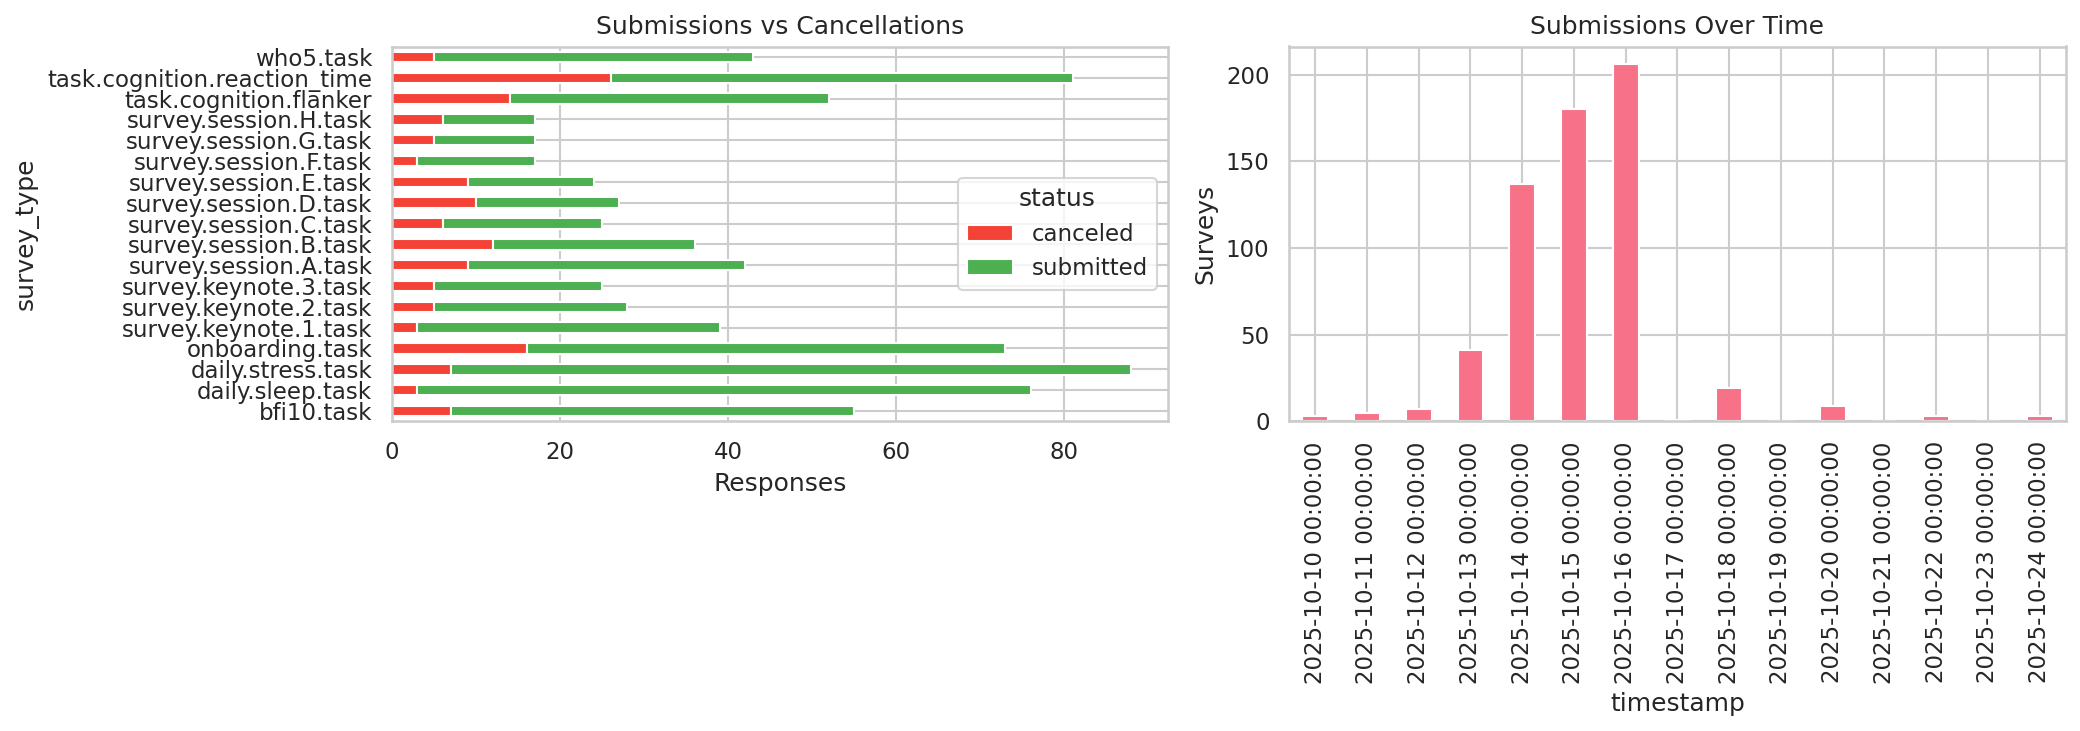
\includegraphics[width=\textwidth]{figures/01_survey_overview.png}
\caption{Survey submission status and temporal distribution of responses.}
\label{fig:survey_overview}
\end{figure}

\begin{table}[ht]
\centering
\caption{Survey instruments and response counts.}
\label{tab:surveys}
\small
\begin{tabular}{lrr}
\toprule
\textbf{Survey Type} & \textbf{Submitted} & \textbf{Participants} \\
\midrule
Daily stress          &  70 & 36 \\
Daily sleep           &  64 & 36 \\
Onboarding (demographics) & 39 & 38 \\
Cognition: reaction time & 52 & 26 \\
BFI-10 (Big Five)     &  44 & 42 \\
Cognition: Flanker    &  35 & 23 \\
WHO-5 (wellbeing)     &  37 & 37 \\
Session ratings (A--H) & 129 & 7--30 \\
Keynote ratings (1--3) &  76 & 18--35 \\
Offboarding           &  15 & 15 \\
\bottomrule
\end{tabular}
\end{table}

\subsubsection{Demographics}

38~participants completed the onboarding survey (one response each), and all 38 gave valid age data (Figure~\ref{fig:demographics}).
The median age was 30~years (mean~33.1, range 23 to 58), with both junior and senior researchers represented.
57.9\% were male ($n=22$) and 42.1\% female ($n=16$).

In terms of academic roles, students made up 57.9\% ($n=22$), professors 21.1\% ($n=8$), postdocs 15.8\% ($n=6$), and researchers 5.3\% ($n=2$).
More than half of the participants (57.9\%, $n=22$) were at UbiComp for the first time, while 23.7\% had been to 4 to 6 previous editions and 7.9\% had attended 7 or more.

\begin{figure}[H]
\centering
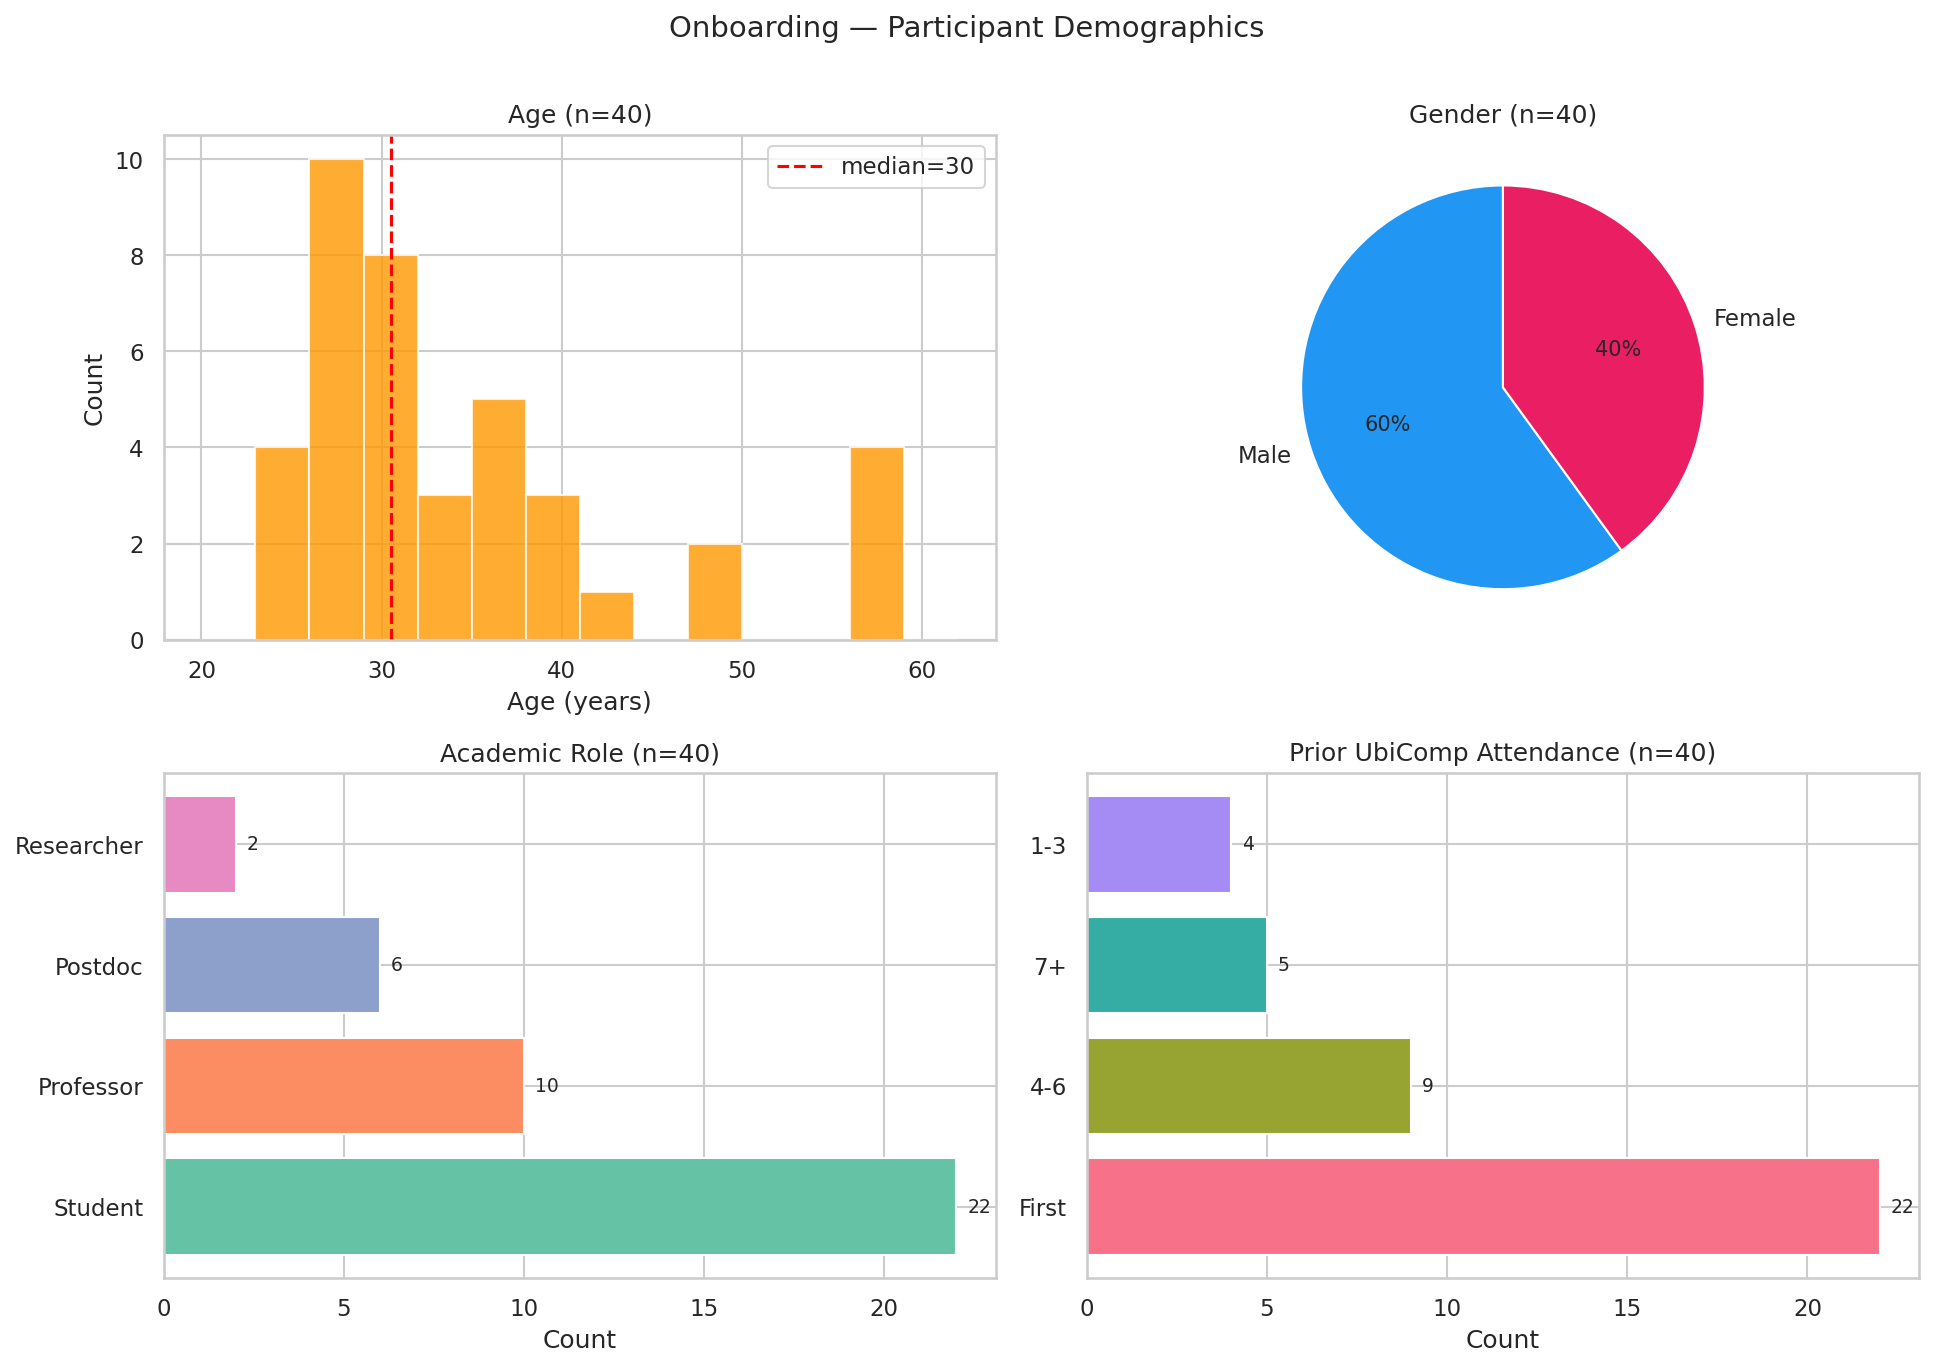
\includegraphics[width=\textwidth]{figures/01_demographics.png}
\caption{Participant demographics: age distribution, gender, academic role, and prior UbiComp experience.}
\label{fig:demographics}
\end{figure}

\subsubsection{Wellbeing: WHO-5}

37~participants completed the WHO-5 Well-Being Index (Figure~\ref{fig:who5_bfi10}, left panel).
Scores ranged from 28\% to 84\%, with a median of 60\% and a mean of 57.4\%.
10~participants (27.0\%) scored below the 50\% threshold that is used to screen for depression risk~\cite{topp2015who5}.
In the general population, this proportion is typically around 15 to 20\%, so the higher rate here could be related to the travel, time pressure, and irregular schedules that come with attending a conference.

\subsubsection{Personality: BFI-10}

The BFI-10 (Big Five Inventory, 10-item short form)~\cite{rammstedt2007bfi10} was completed by 42~participants (Figure~\ref{fig:who5_bfi10}, right panel).
Table~\ref{tab:bfi10} summarises the five personality dimensions (scale 0--4).

\begin{figure}[H]
\centering
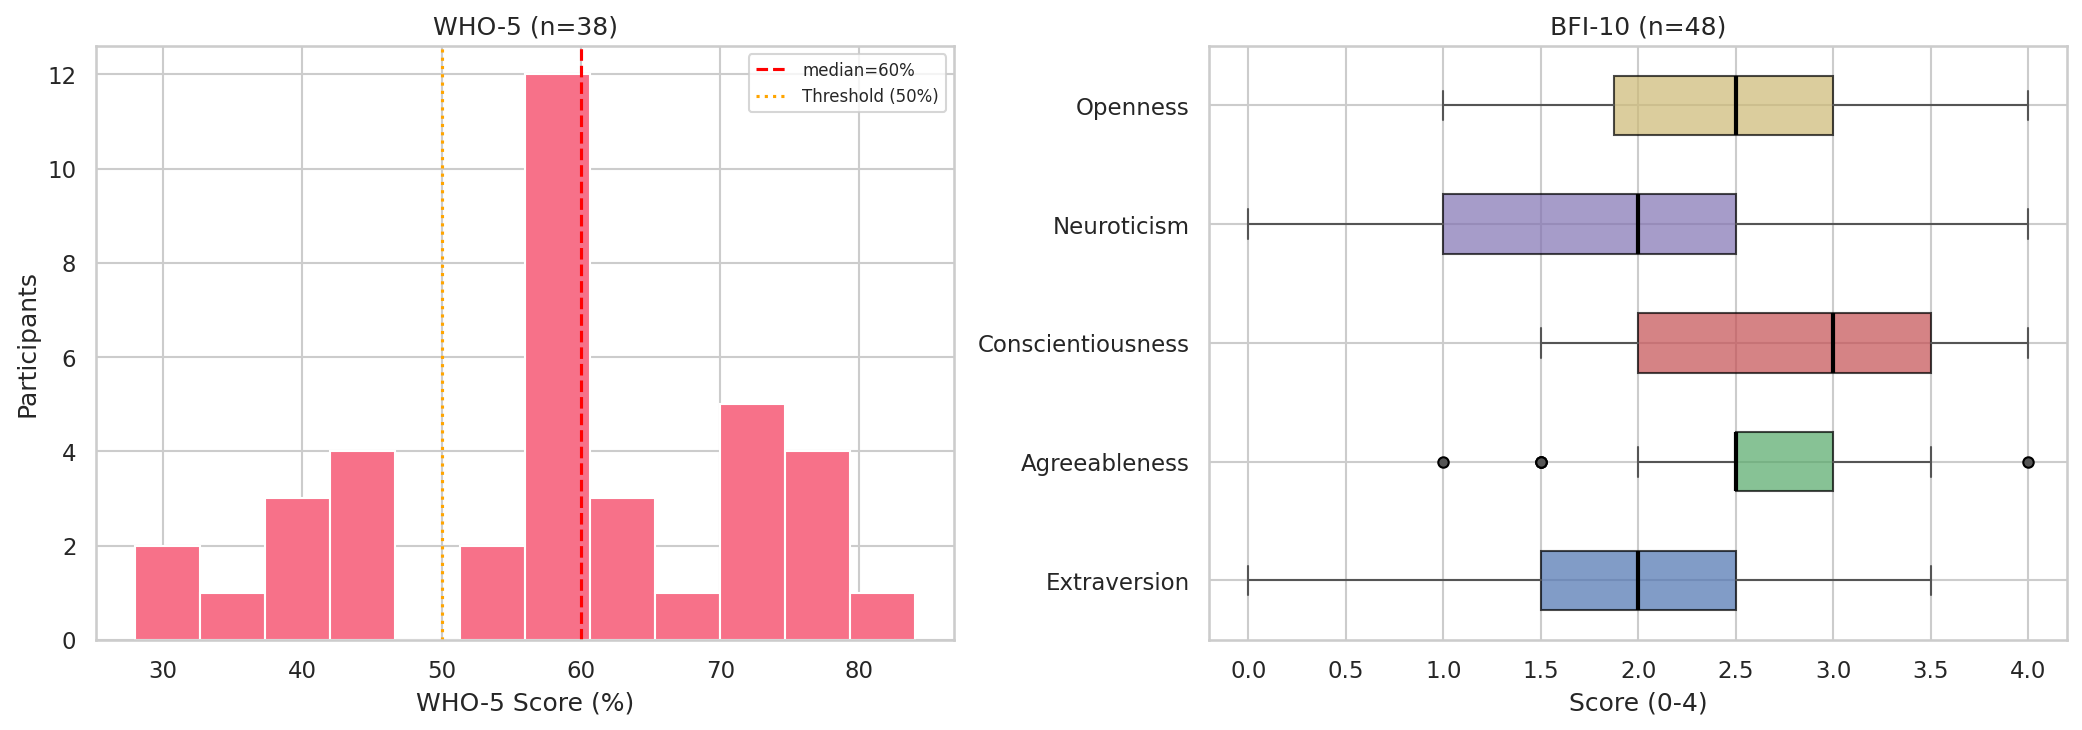
\includegraphics[width=\textwidth]{figures/01_who5_bfi10.png}
\caption{Left: WHO-5 wellbeing score distribution ($n=37$); dashed line marks the 50\% at-risk threshold. Right: BFI-10 personality dimension distributions ($n=42$).}
\label{fig:who5_bfi10}
\end{figure}

\begin{table}[ht]
\centering
\caption{BFI-10 personality dimension scores ($n=42$, scale 0--4).}
\label{tab:bfi10}
\small
\begin{tabular}{lcc}
\toprule
\textbf{Dimension} & \textbf{Mean} & \textbf{Std} \\
\midrule
Conscientiousness & 2.74 & 0.73 \\
Agreeableness     & 2.68 & 0.62 \\
Openness          & 2.42 & 0.71 \\
Extraversion      & 2.07 & 0.76 \\
Neuroticism       & 1.92 & 0.85 \\
\bottomrule
\end{tabular}
\end{table}

Conscientiousness had the highest mean score (2.74), which makes sense for an academic sample.
Neuroticism was the lowest (mean~1.92) but also had the widest spread (std~0.85), so there was quite a bit of variation between participants.
Extraversion scores were moderate (mean~2.07), meaning the group included both outgoing and more reserved people.

\subsubsection{Daily Stress and Sleep}

Daily stress was reported on a 0 to 10 scale, with 70~responses from 36~participants (Figure~\ref{fig:daily_surveys}).
The median stress level was 4.0 (mean~4.3, range 1 to 10), so stress was moderate on average.

For sleep quality ($n=64$), most responses were positive: 51.6\% said ``Good'', 26.6\% ``Neutral'', 14.1\% ``Bad'', 4.7\% ``Very Bad'', and 3.1\% ``Amazing''.
Sleep duration paints a different picture though: 43.8\% reported sleeping fewer than 6~hours, 51.6\% slept 6 to 8~hours, and only 4.7\% got more than 8~hours.
So while people felt their sleep was okay, many of them were actually not getting enough hours, which is not unusual during a conference week.

\begin{figure}[H]
\centering
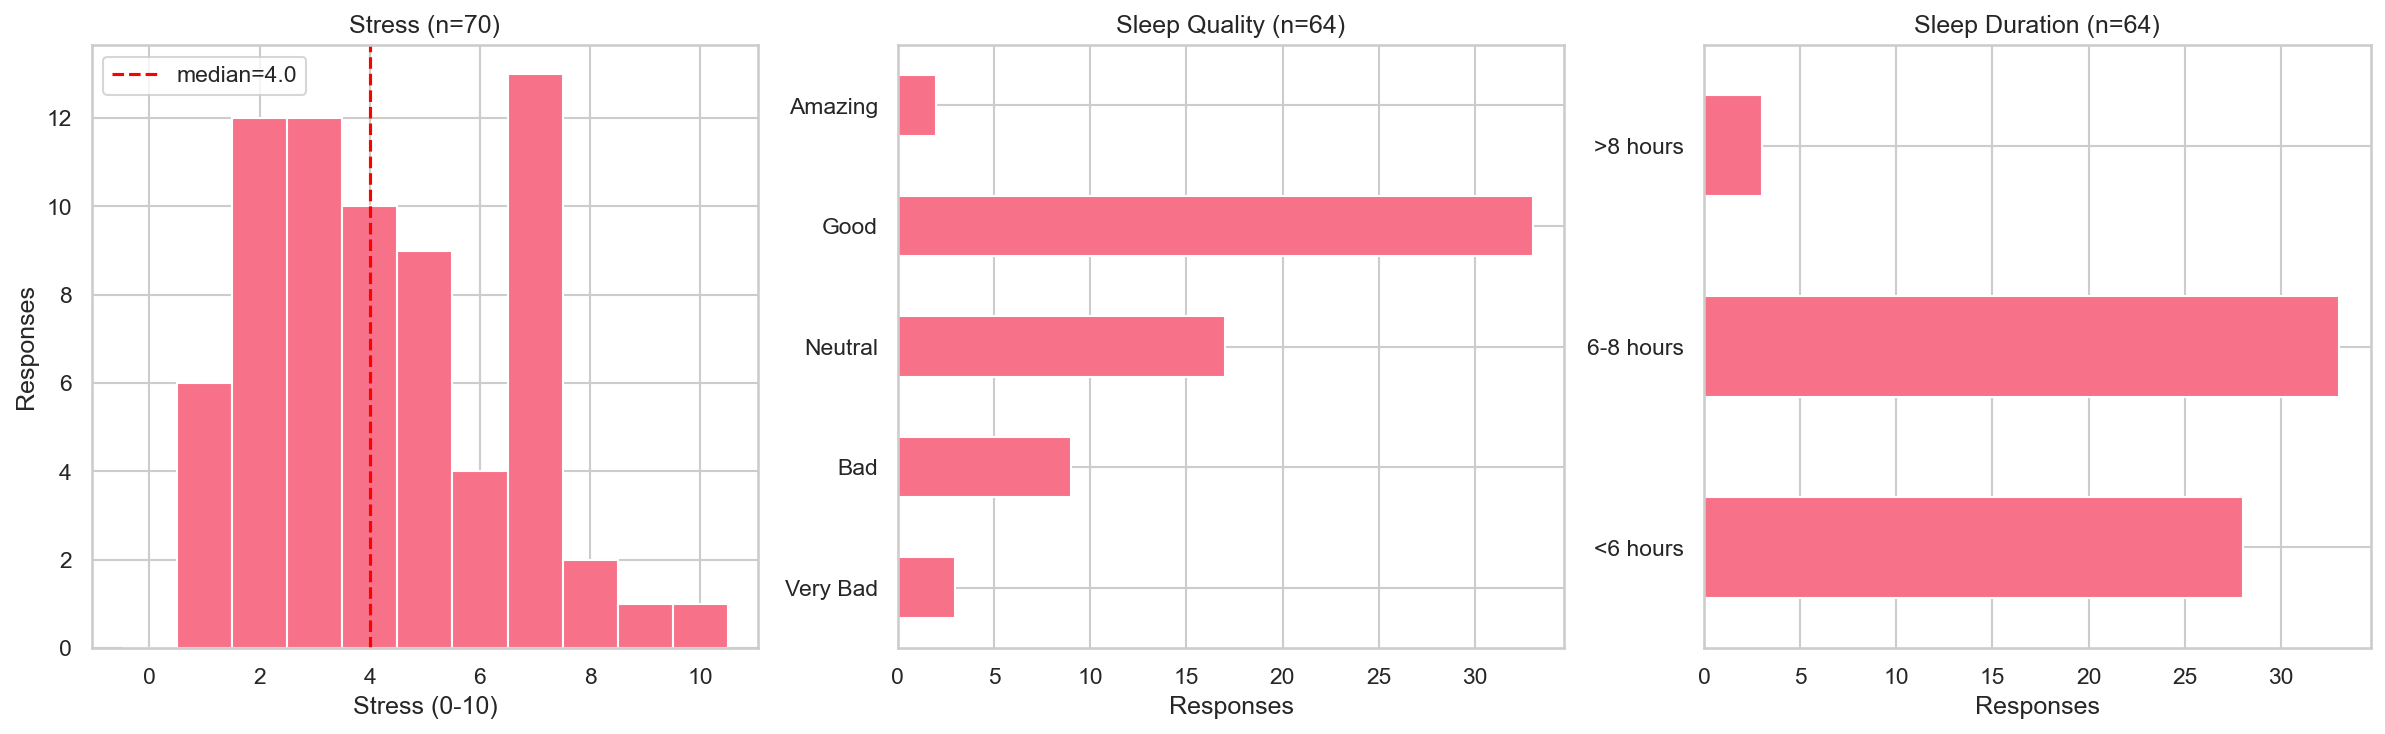
\includegraphics[width=\textwidth]{figures/01_daily_surveys.png}
\caption{Daily self-report distributions: stress level (0--10), sleep quality, and sleep duration.}
\label{fig:daily_surveys}
\end{figure}

% ============================================================
\section{Data Preparation}
% ============================================================

\subsection{Filtering to Conference Period}

Timestamps were converted from UTC to local conference time (Europe/Helsinki) before filtering and any time-of-day analysis.
All streams were filtered to the main conference week (October~13 to 16, 2025, local time).
How much data was kept depends on the stream: screen events kept 99.1\%, step count 87.9\%, activity 83.3\%, location 70.0\%, heartbeat 51.9\%, and ambient light 64.0\%.

\subsection{Step-Count Processing}

Raw cumulative pedometer values were converted to per-interval step deltas:
\begin{enumerate}
    \item Compute the first difference of the cumulative counter per participant.
    \item Clip negative values (counter resets) to zero; fill NaN with zero.
\end{enumerate}

\subsection{Survey Parsing}

The raw survey responses were stored as JSON columns with nested answer structures after parquet conversion.
The protocol reuses the \texttt{onboarding.task} identifier for the offboarding survey, so offboarding responses were separated by their answer fields, and duplicate uploads (same participant, timestamp and survey) were removed.
We wrote custom parsers to extract values and text labels for each survey type:
\begin{itemize}
    \item \textbf{Onboarding}: age, gender, academic role, prior conference experience.
    \item \textbf{Daily stress}: single 0 to 10 Likert scale per day.
    \item \textbf{Daily sleep}: quality (categorical) and duration (categorical).
    \item \textbf{WHO-5}: five items scored 0 to 5; raw sum $\times$ 4 = percentage (0 to 100).
    \item \textbf{BFI-10}: ten items with reverse coding on selected dimensions; scores on five personality traits (0 to 4).
    \item \textbf{Event ratings}: session (A--H) and keynote (1--3) ratings with attendance confirmation.
    \item \textbf{Cognition}: reaction time (average reaction time, correct and wrong taps) and Flanker (score, swipes, mean congruent/incongruent response times); one row per test.
\end{itemize}

\subsection{Processed Outputs}

The processed data is about 22\,MB across 17~Parquet files.
Tables~\ref{tab:processed_sensor} and~\ref{tab:processed_survey} list each file with its row count and columns.
All sensor tables have common metadata columns (\texttt{participant\_id}, \texttt{timestamp}, \texttt{sequenceId}, \texttt{studyDeploymentId}, \texttt{deviceRoleName}, \texttt{syncPoint.*}, \texttt{dataStream.*}). Below we only list the data columns specific to each stream. Note that sensor columns use the original CARP naming with a \texttt{measurement.data.} prefix (e.g.\ the full column name for \texttt{batteryLevel} is \texttt{measurement.data.batteryLevel}), while survey tables use cleaned snake\_case names without any prefix.

\begin{table}[H]
\centering
\caption{Processed sensor Parquet files (conference period, October~13--16).}
\label{tab:processed_sensor}
\small
\begin{tabular}{lrrl}
\toprule
\textbf{File} & \textbf{Rows} & \textbf{Part.} & \textbf{Data Columns} \\
\midrule
\texttt{stepcount}
    & 393\,300 & 77
    & \texttt{steps\_cumulative}, \texttt{steps\_delta} \\
\texttt{activity}
    & 166\,047 & 77
    & \texttt{type}, \texttt{confidence} \\
\texttt{location}
    &  93\,209 & 78
    & \texttt{latitude}, \texttt{longitude}, \texttt{altitude}, \texttt{speed}, \\
    & & & \texttt{heading}, \texttt{accuracy}, \texttt{speedAccuracy} \\
\texttt{heartbeat}
    & 106\,244 & 80
    & \texttt{period}, \texttt{deviceType}, \texttt{deviceRoleName} \\
\texttt{weather}
    &   3\,050 & 65
    & \texttt{temperature}, \texttt{tempMin}, \texttt{tempMax}, \\
    & & & \texttt{humidity}, \texttt{pressure}, \texttt{windSpeed}, \\
    & & & \texttt{cloudiness}, \texttt{weatherMain}, \texttt{rainLastHour} \\
\texttt{airquality}
    &   3\,033 & 65
    & \texttt{airQualityIndex}, \texttt{airQualityLevel} \\
\texttt{batterystate}
    &  13\,263 & 58
    & \texttt{batteryLevel}, \texttt{batteryStatus} \\
\texttt{screenevent}
    &   5\,606 & 22
    & \texttt{screenEvent} (ON / OFF / UNLOCKED) \\
\texttt{ambientlight}
    &   1\,993 & 19
    & \texttt{meanLux}, \texttt{minLux}, \texttt{maxLux}, \texttt{stdLux} \\
\bottomrule
\end{tabular}
\end{table}

\begin{table}[H]
\centering
\caption{Processed survey and cognition Parquet files (one table per survey type).}
\label{tab:processed_survey}
\small
\begin{tabular}{lrrl}
\toprule
\textbf{File} & \textbf{Rows} & \textbf{Part.} & \textbf{Columns} \\
\midrule
\texttt{survey\_onboarding}
    & 38 & 38
    & \texttt{participant\_id}, \texttt{timestamp}, \texttt{age}, \\
    & & & \texttt{gender\_value}, \texttt{gender\_text}, \\
    & & & \texttt{academic\_value}, \texttt{academic\_text}, \\
    & & & \texttt{prior\_value}, \texttt{prior\_text}, \texttt{presenter\_texts} \\
\texttt{survey\_daily\_stress}
    & 70 & 36
    & \texttt{participant\_id}, \texttt{date}, \texttt{timestamp}, \\
    & & & \texttt{stress\_level} \\
\texttt{survey\_daily\_sleep}
    & 64 & 36
    & \texttt{participant\_id}, \texttt{date}, \texttt{timestamp}, \\
    & & & \texttt{sleep\_quality\_value}, \texttt{sleep\_quality\_text}, \\
    & & & \texttt{sleep\_hours\_value}, \texttt{sleep\_hours\_text} \\
\texttt{survey\_who5}
    & 37 & 37
    & \texttt{participant\_id}, \texttt{timestamp}, \\
    & & & \texttt{q1}, \texttt{q2}, \texttt{q3}, \texttt{q4}, \texttt{q5}, \\
    & & & \texttt{raw\_sum}, \texttt{pct\_score} \\
\texttt{survey\_bfi10}
    & 42 & 42
    & \texttt{participant\_id}, \texttt{timestamp}, \\
    & & & \texttt{extraversion}, \texttt{agreeableness}, \\
    & & & \texttt{conscientiousness}, \texttt{neuroticism}, \texttt{openness} \\
\texttt{survey\_event\_ratings}
    & 205 & 38
    & \texttt{participant\_id}, \texttt{timestamp}, \\
    & & & \texttt{attending\_text}, \texttt{rating\_value}, \texttt{rating\_text}, \\
    & & & \texttt{event\_type}, \texttt{event\_id} \\
\texttt{cognition\_reaction\_time}
    & 52 & 26
    & \texttt{participant\_id}, \texttt{date}, \texttt{timestamp}, \\
    & & & \texttt{avg\_reaction\_time\_ms}, \texttt{correct\_taps}, \texttt{wrong\_taps} \\
\texttt{cognition\_flanker}
    & 35 & 23
    & \texttt{participant\_id}, \texttt{date}, \texttt{timestamp}, \texttt{score}, \texttt{time}, \\
    & & & \texttt{right\_swipes}, \texttt{wrong\_swipes}, \\
    & & & \texttt{mean\_congruent\_ms}, \texttt{mean\_incongruent\_ms}, \\
    & & & \texttt{n\_congruent}, \texttt{n\_incongruent} \\
\bottomrule
\end{tabular}
\end{table}

\subsection{Data Quality Notes}

\begin{itemize}
    \item \textbf{Heartbeat gaps}: mean coverage of 33.4\% during the conference indicates frequent device disconnections.
    \item \textbf{Night-time blind spots}: all sensors show $\sim$50\% lower coverage after midnight.
    \item \textbf{Per-participant variance}: step-count records range from $<$1\,000 to $>$30\,000 across participants.
\end{itemize}

% ============================================================
% References
% ============================================================
\begin{thebibliography}{9}
\bibitem{ubicomp2025}
ACM, \emph{UbiComp/ISWC 2025}, Aalto University, Espoo, Finland, October 12--16, 2025.
\url{https://www.ubicomp.org/ubicomp-iswc-2025/}

\bibitem{topp2015who5}
C.~W. Topp, S.~D. {\O}stergaard, S.~S{\o}ndergaard, and P.~Bech,
``The WHO-5 Well-Being Index: A systematic review of the literature,''
\emph{Psychotherapy and Psychosomatics}, vol.~84, no.~3, pp.~167--176, 2015.

\bibitem{rammstedt2007bfi10}
B.~Rammstedt and O.~P. John,
``Measuring personality in one minute or less: A 10-item short version of the Big Five Inventory in English and German,''
\emph{Journal of Research in Personality}, vol.~41, no.~1, pp.~203--212, 2007.
\end{thebibliography}

\end{document}
